\section{Restricted Space Usage Model}
\label{section:usagemodel}

\begin{figure*}[t!]
\centering
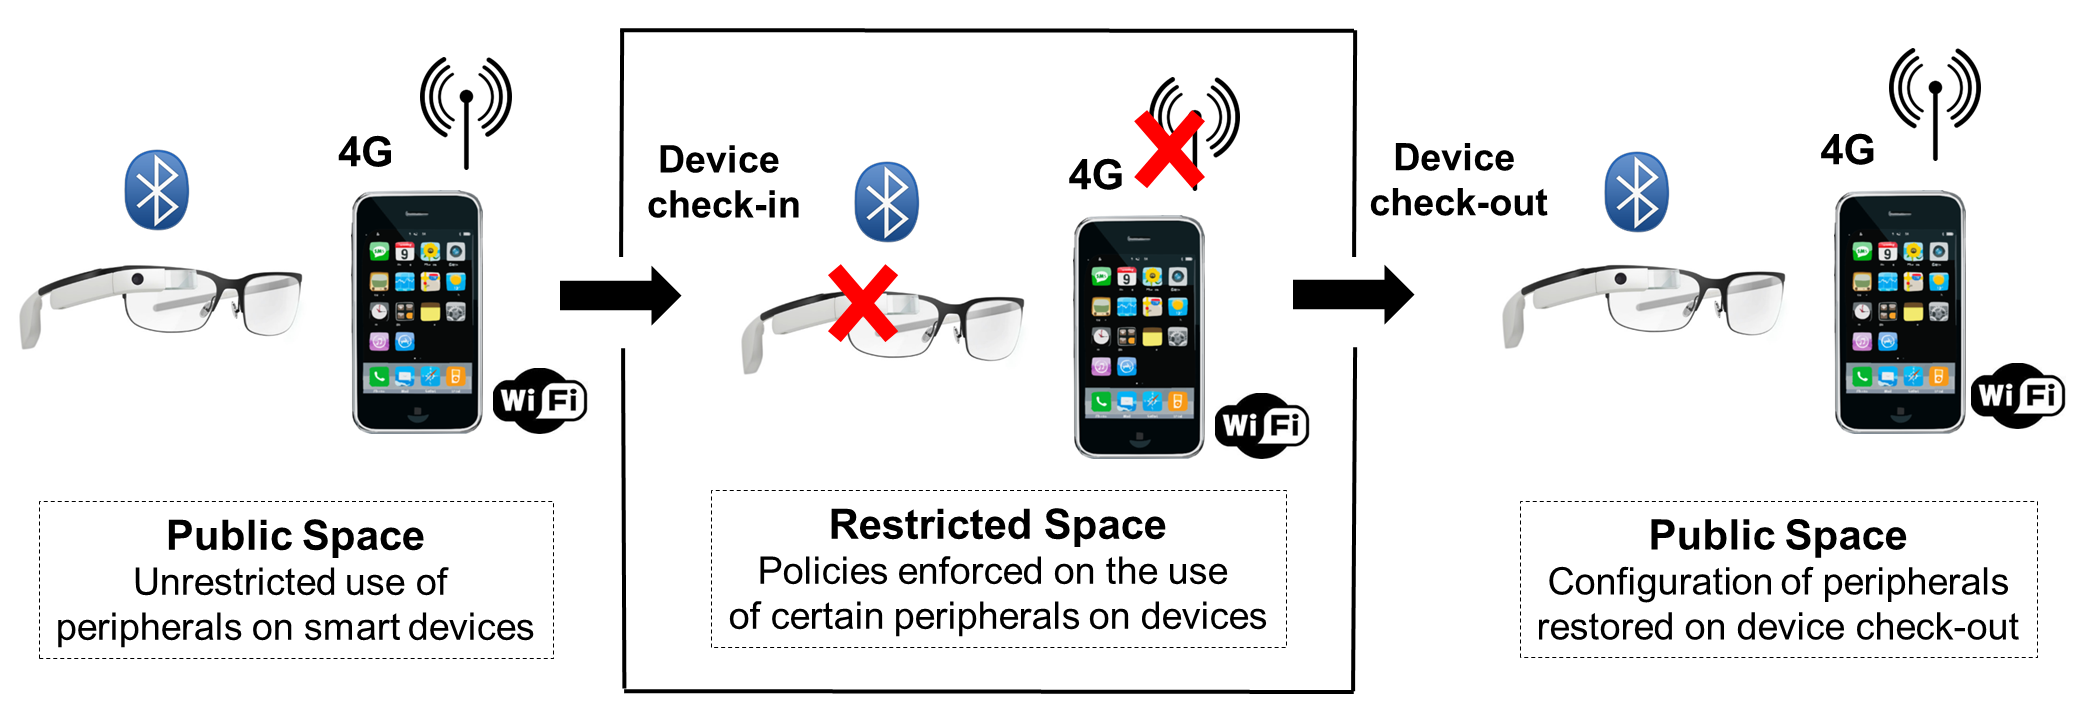
\includegraphics[keepaspectratio=true,width=0.85\textwidth]{figures/restricted-space.png}
\indent\vspace{-0.5cm}
\mycaption{An overview of our restricted space model. Guests ``check-in''
devices when entering restricted spaces. During check-in, hosts inspect,
analyze and modify the configurations of these devices in accordance with their
usage policies. In this example, the host restricts the use of the camera on
the smart glass, and the 4G data interface on the smart phone. However, the
glass can continue to use its Bluetooth interface to pair with the smart phone,
while the phone can use WiFi.  When guests leave the restricted space, they
``check-out'' their devices, which the host then restores to their original
configurations.}
{\label{figure:restrictedspaces}}
\indent\vspace{-0.55cm}
\end{figure*}

We now provide an overview of the restricted space model, motivate some
features of our enforcement mechanism, and describe our threat model.

\subsection{Overall Workflow}

\myparagraph{Check-in}
As depicted in \figref{figure:restrictedspaces}, when a guest enters a
restricted space in which he wishes to use his devices, he ``checks-in'' each
of his devices during entry. During check-in, the guest device communicates
with the host's policy server to perform the following tasks:

\begin{mylist}
%
\item \textit{Authentication.} The authentication step allows the guest and
host to mutually identify each other. We assume that both the guest and the
host have cryptographic credentials (\eg~public/private key pairs) that can be
validated via a trusted third party, such as a certifying authority. The host
and the guest mutually authenticate each other's credentials in the standard
way, for example, as is typically done during SSL/TLS handshakes.

The host's policies are enforced by a mechanism that executes in the guest.  As
previously discussed, this mechanism is part of the TCB, and must therefore not
be tampered by the guest.  We rely on secure hardware on the guest device (the
ARM TrustZone) to ensure this property.  In particular, we rely on the secure
hardware to detect and prevent any attempts to tamper with the TCB on the
guest. This can be ensured using a special boot-time protocol implemented atop
the secure hardware.

It is important to note that this TCB is \textit{not} the end-user's usual work
environment on the device, \eg~the traditional Android, iOS or Windows
environment with apps. Rather, the TCB is an environment that is created and
distributed by a trusted entity, such as the device vendor, and executes in
isolation on the guest device. 

% NOTE: Clarification from Ferdinand -- this is not how attestation works on
% the TZ as there is no hardware root of trust on the device. Rather vendors
% lock down the secure world and implement secure boot within it.
%
% The host checks the trustworthiness of the TCB by attesting the software
% stack that executes the policy enforcement mechanism.  This attestation is
% typically done from the hardware-up, and is used to ensure that the TCB
% booted correctly and only executes software components that can be trusted by
% the host.  
%
% We can therefore assume that the correct configurations of the TCB are
% well-known to the host, thereby enabling attestation. As we will describe in
% \sectref{section:mechanism}, our TCB on guest devices is simple in its
% functionality and small in size. We attest this TCB using trusted hardware on
% the guest device (the ARM TrustZone) as the root of trust, but other
% implementations may be possible.

\item \textit{Host analyzes device.} The host leverages the TCB to analyze the
guest device. Our mechanism allows hosts to \textit{remotely fetch memory
pages} (and CPU register state) belonging to the guest device.  The TCB
computes a cryptographic checksum over the memory pages to ensure that they are
not tampered with as they are transferred from the guest to the host. 

The host uses raw memory pages from the device in two ways. First, it scans
memory pages to ensure that the device is free of malicious software, \eg~in
the form of malicious apps or kernel modules.  Second, it extracts
configuration information from the device. This includes the kernel version,
the list of peripherals supported by the device, memory addresses of various
device drivers for peripherals on the device and the state of these peripherals
(\eg~whether a certain peripheral is enabled and its settings). The host can
also checkpoint the state of these peripherals so that they can be restored at
check-out. 

\item \textit{Host modifies guest's configuration.} The host modifies the guest
device's configuration to conform to its restricted usage policies.  In the
example shown in \figref{figure:restrictedspaces}, the host's policy is to
disable the camera and the 3G/4G data plan on all devices. The host enforces
this policy by creating a sequence of \textit{remote memory writes} that
directly modify the memory state of the device. For example, the host could
prevent the use of the camera and 3G/4G data plan by unlinking the device
drivers corresponding to the camera and the modem. The host uses the
configuration information extracted in the previous step to determine the
memory addresses that must be modified to unlink these drivers. 

We assume that it is the host's responsibility to ensure that these
configuration modifications are not easily bypassable. For example, these
modifications may be undone if the user of the guest device can directly modify
kernel memory, \eg~by dynamically loading kernel modules or using
\code{/dev/kmem} in the end-user's work environment. The host must use the
inspection phase to identify device configurations that could lead to such
attacks, and disallow the use of such devices in the restricted space.

\item \textit{Host obtains verification token from guest.} After the guest
device has been configured, the TCB produces a \textit{verification token} to
be transmitted to the host. The verification token is an unforgeable value that
encapsulates the set of configuration changes to the device. The TCB computes
the token as a checksum over the memory locations that were modified.  The
token is unforgeable in that only the TCB can re-create its value as long as
the device configuration has not been altered, and any malicious attempts to
modify the token can be detected by the TCB and the host.

At any point when the device is in the restricted space, the host can request
the TCB on the device to send it the verification token. The TCB computes this
token afresh, and transmits it to the host,\footnote{This assumes that the
host's policy still allows a communication channel between the host and the
guest. If all of the guest's peripherals are disabled, the host will need
physical access to the guest to visually obtain the freshly-computed
verification token.} which compares this freshly-computed token with the one
obtained during check-in. It can use this comparison to ensure that the guest
has not altered the device configurations from the previous step.  The
verification token is ephemeral, and can be computed afresh by the guest only
within an expiration period.  In our prototype, the TCB cannot recompute the
verification token if the guest device is rebooted, thereby ensuring that
end-users cannot undo the host's configuration changes by simply rebooting the
device.
%
\end{mylist}

\myparagraph{Check-out}
Once checked-in, the guest device can freely avail of the facilities of the
restricted space under the policies of the host. For example, in
\figref{figure:restrictedspaces}, the smart glass can pair with the smart phone
via Bluetooth, while the smart phone can connect to and use the host's WiFi
access point. When the guest exits the restricted space, he checks-out the
device, accomplishing two goals: 
%
\begin{mylist}
%
\item \textit{Host checks guest state.} The host checks guest device's
configuration by requesting the verification token from the device's TCB to
ensure that the configuration has not been altered. If it finds that the
verification token does not match the value obtained from the device at
check-in, it can detain the device for further inspection, \eg~to determine
whether any data from the restricted environment was exfiltrated.

Note that it is not usually possible to differentiate between mismatches that
happen because of benign reasons, such as a device reboot, or malicious ones,
such as when an end-user intentionally modified the peripheral configurations
required by the host. This is because even malicious modifications can be
masked by simply rebooting the device, and making the mismatch seem benign.
Thus, the host's policy to deal with mismatches depends upon the sensitivity of
the restricted environment. For example, in a federal setting, a detailed
forensic examination of the device may be necessary, the possibility of which
could deter a malicious guest from bypassing the host's policy enforcement. As
previously discussed, hosts can request the verification token from the device
at any time when it is in the restricted space. Hosts can use this feature to
frequently check the verification token and narrow down the timeframe of the
violation.

\item \textit{Restoring guest state.} To restore the state of the device, the
end-user could simply reboot the device. The host only modifies the memory of
the device, and not persistent storage. Rebooting therefore undoes all the
memory modifications performed by the host and boots the device from an
unmodified version of the kernel in persistent storage. Alternatively, the host
can restore the state of the guest device's peripherals from a checkpoint
created at check-in. The main challenge here is to ensure consistency between
the state of a peripheral and the view of the peripheral from the perspective
of user-level apps. For example, when the 3G interface is disabled, an app
loses network connectivity. However, because we only modify memory and do not
actually reset the peripheral, the 3G card may have accumulated packets, which
the app may no longer be able to process when the kernel state is restored.
Mechanisms such as shadow drivers~\cite{shadow:tocs06} can enable such ``hot
swaps'' of kernel state, enabling the guest device to continue without
rebooting.
%
\end{mylist}

% \todo{VG}{A security analysis here? -- No need. Fold in any security
% arguments with the corresponding step in the workflow.}

\subsection{Malicious Hosts} 
\label{section:usagemodel:malicious}
%
Our discussion so far has assumed that hosts are benign. Authentication at
check-in ensures that remote access to guest device memory is available only to
hosts that the guest approves. However, it may be possible even for such hosts
to misuse the facilities of our mechanism to violate the security and privacy
of the guest. For example, a malicious host could use remote memory reads to
obtain the guest's personal data. It could also install a key logger or a
backdoor to spy on the guest's activities. Even if the host is not overtly
malicious, it is possible that the configuration changes that it makes will
render the guest's device vulnerable to attacks. This is reminiscent of the
2006 incident when CD DRM software installed by Sony made the systems on which
it was installed vulnerable to certain kinds of attacks~\cite{sonydrm:sec06}.

To protect guest devices from malicious hosts, we provide a \textit{trusted
vetting service}. We assume that guests register their device(s) with the
vetting service beforehand. When the host sends a remote read/write request,
the guest device forwards the request to the service together with its current
memory configuration. The vetting service analyzes the requests against the
memory configuration and determines whether the request conforms to certain
safety policies. \sectref{section:vetting} presents the details of our vetting
service.

The vetting service could directly be implemented in the TCB executing on the
guest device, but this has the undesirable effect of bloating the TCB on the
device. We therefore implement vetting as a cloud service.  Note that vetting
is optional. If the guest trusts the host, it could carry out the host's
requests without vetting.

% It is challenging to protect guest devices from malicious hosts, and
% \textit{for this paper, we will assume that hosts are benign}. Nevertheless,
% there are a few defenses that could be used to protect against malicious
% hosts.  To protect personal data, privacy-conscious users could store their
% data encrypted on disk and in memory, except when it is used. However, this
% would require apps on the device to be redesigned to be aware of such
% encrypted data.

% To protect against remote writes that maliciously modify the guest device
% (\eg~by installing a keylogger), the guest could rely on a trusted third
% party to vet the operations of the host. That is, the guest could forward its
% memory configuration and the remote operations requested by the host to the
% trusted third party prior to making any memory modifications. The guest would
% proceed with the modifications only if the trusted third party certifies that
% the operations do not install malicious software on the guest device.
% Alternatively, a simpler solution is to restrict the kinds of remote write
% operations that a host can initiate. For example, the TCB could enforce that
% the only remote memory writes available to the host are writing \textsc{null}
% bytes to memory locations that store device driver hooks. This would allow
% hosts to unlink drivers and disable peripherals, but prevent them from
% installing malicious software.

\subsection{Covert Use of Devices}
%
It is certainly possible for a guest to bypass the host's policies by not
declaring a device during check-in. As long as the guest carefully configures
the device to avoid accessing any of the host's resources in the restricted
space, \eg~its WiFi access points, and remain stealthy, the device cannot be
detected by the host.

Our focus in this paper is to address policy enforcement for \textit{overt}
uses of smart devices. \textit{Covert} uses, such as the above, are out of the
scope of the mechanisms developed in this paper. Instead, we assume that
traditional methods such as physical security checks are necessary to detect
covertly-hidden devices.

\subsection{Threat Model} 
\label{section:threat}
%
Given the discussion in this section, we now summarize our threat model. 
Each guest device is assumed to be partitioned into two parts: (1)~the
end-user's work environment, and (2)~the environment that runs the policy
enforcement mechanism (part of the TCB). 

From the perspective of the host, the end-user's work environment is untrusted.
The host must trust the policy enforcement mechanism, but because it executes
on the guest device, the host leverages secure hardware, the ARM TrustZone in
our case, to bootstrap this trust. Having established trust, the host then uses
the policy enforcement mechanism to securely read and modify the memory state
of the work environment. It is the host's responsibility to inspect the memory
state of the work environment to determine whether it is malicious, contains
known exploitable vulnerabilities, or allows guests to bypass the configuration
changes that the host may make.  Once the host determines that the guest's work
environment is acceptable, it can induce changes to the guest's memory state.
Guests are assumed to keep their devices powered on for the duration of their
stay in the restricted space, failing which the verification tokens will no
longer match. Mismatches may also happen if the guest maliciously modifies the
host's changes.

The work environment may contain zero-day vulnerabilities, such as a
newly-discovered buffer overflow in the kernel. The host may not be aware of
this vulnerability, but a malicious guest may know of it and have an exploit to
bypass the host's policies.  Such threats are outside the scope of our work,
but the host may protect itself by requiring the guest's work environment to
run a fortified software stack (\eg~Samsung Knox~\cite{knox:ccs14} or
MOCFI~\cite{mocfi:ndss12}). The host can check this requirement during the
inspection phase. A malicious work environment may also launch a
denial-of-service attack, which will prevent the host from communicating with
the TCB on the guest device.  However, such attacks can readily be detected by
the host, which can then prevent the device from entering the restricted space.
We therefore exclude such attacks from our threat model.

From the perspective of the guest, if the host is untrusted, it can rely on a
trusted vetting service to determine if the host's read and write requests are
safe.

% the host is assumed to only make benign changes to the guest work
% environment.  However, it may be possible to relax this assumption provided
% the guest vets all the host's intended changes with a trusted third party.
% Similarly, although the host is assumed not to maliciously compromise the
% guest's privacy, a guest may choose to encrypt its in-memory and on-disk data
% to protect it from the host.


% What if kernel module is loaded dynamically? We disable that.



